\documentclass[a2paper, 12pt]{article}
\usepackage[font={huge, bf}]{caption}
\usepackage{fontspec}
\setmainfont{Arial}
\usepackage{subcaption}
\usepackage{graphicx}
\usepackage{tikz}
\usepackage{tikzsymbols}
\usetikzlibrary{calc,patterns,shapes.geometric}
\usepackage{float}
\usepackage{pdflscape}
\usepackage{geometry}
\geometry{landscape, margin=2cm}
\captionsetup[subfigure]{justification=justified,singlelinecheck=false}
\pagestyle{empty}

\def\centerarc[#1](#2)(#3:#4:#5){\draw[#1] ($(#2)+({#5*cos(#3)},{#5*sin(#3)})$) arc (#3:#4:#5);}

\begin{document}
	\vspace*{\fill}
	\begin{figure}[!htbp]
		\centering
		\begin{subfigure}[b]{0.48\textwidth}
			\caption{Figure 1}
			\centering
			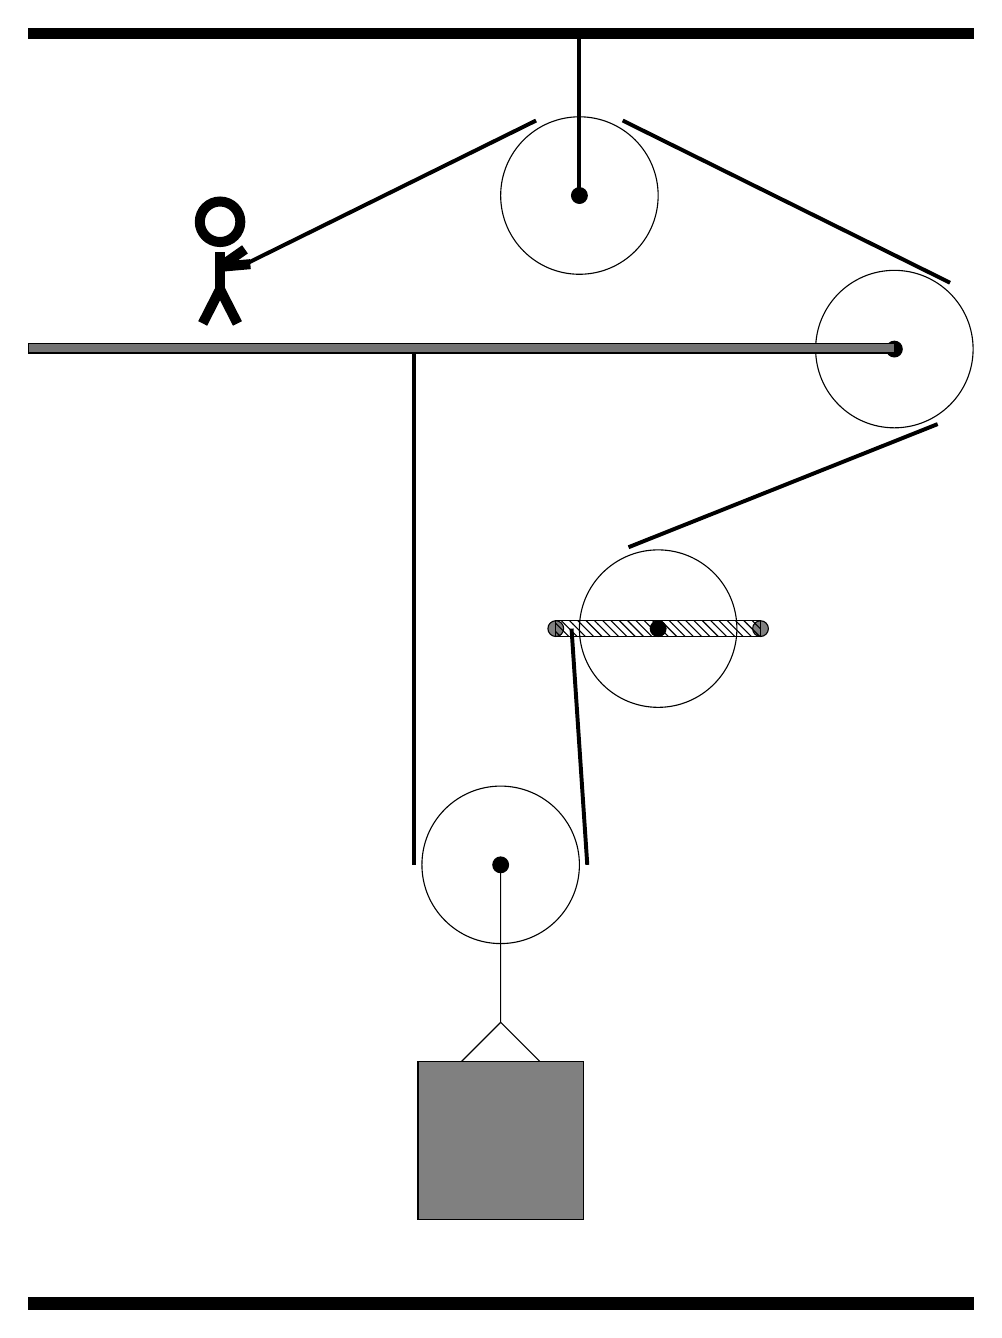
\begin{tikzpicture}
				\draw[fill=black] (-4, 14) rectangle (8, 14.125);
				
				\draw (2, 3.5) circle (1);
				\draw[fill=black] (2, 3.5) circle (0.1);
				
				\draw (7, 10.05) circle (1);
				\draw[fill=black] (7, 10.05) circle (0.1);
				
				\draw[fill=white](4, 6.5) circle (1);
				\draw[fill=black] (4, 6.5) circle (0.1);
				\draw[fill=black!50] (2.7, 6.5) circle (0.1);
				\draw[fill=black!50] (5.3, 6.5) circle (0.1);
				\draw[pattern=north west lines, pattern color=black] (2.7, 6.6) rectangle (5.3, 6.4);
				
				\draw (3, 12) circle (1);
				\draw[fill=black] (3, 12) circle (0.1);
				\draw[line width=0.5mm] (3, 12) -- (3, 14);
				
				\draw (2, 3.5) -- (2, 1.5) -- (1.5, 1.0) -- (2.5, 1.0) -- (2, 1.5);
				\draw[fill=black!50] (0.95, 1.0) rectangle (3.05, -1.0);
				
				\draw[line width=0.5mm] (0.9, 10) -- (0.9, 3.5);
				\centerarc[line width=0.5mm](2, 3.5)(180:360:1.1);
				\draw[line width=0.5mm](3.1, 3.5) -- (2.9, 6.5);
				\centerarc[line width=0.5mm](4, 6.5)(110:180:1.1);
				\draw[line width=0.5mm](3.6238, 7.5337) -- (7.55, 9.0974);
				\centerarc[line width=0.5mm](7, 10.05)(-60:50:1.1);
				\draw[line width=0.5mm](7.7071, 10.8926) -- (3.55, 12.9526);
				\centerarc[line width=0.5mm](3, 12)(60:120:1.1);
				\draw[line width=0.5mm](2.45, 12.9526) -- (-1.2, 11.15);
				
				\node at (-1.5, 11.15) {\footnotesize \scriptsize \Strichmaxerl[10][-175][35]};
				\draw[fill=black!55] (-4, 10) rectangle (7, 10.125);
				
				\draw[fill=black] (-4, -2) rectangle (8, -2.15);
			\end{tikzpicture}
		\end{subfigure}
		\hfill
		\begin{subfigure}[b]{0.48\textwidth}
			\caption{Figure 2}
			\centering
			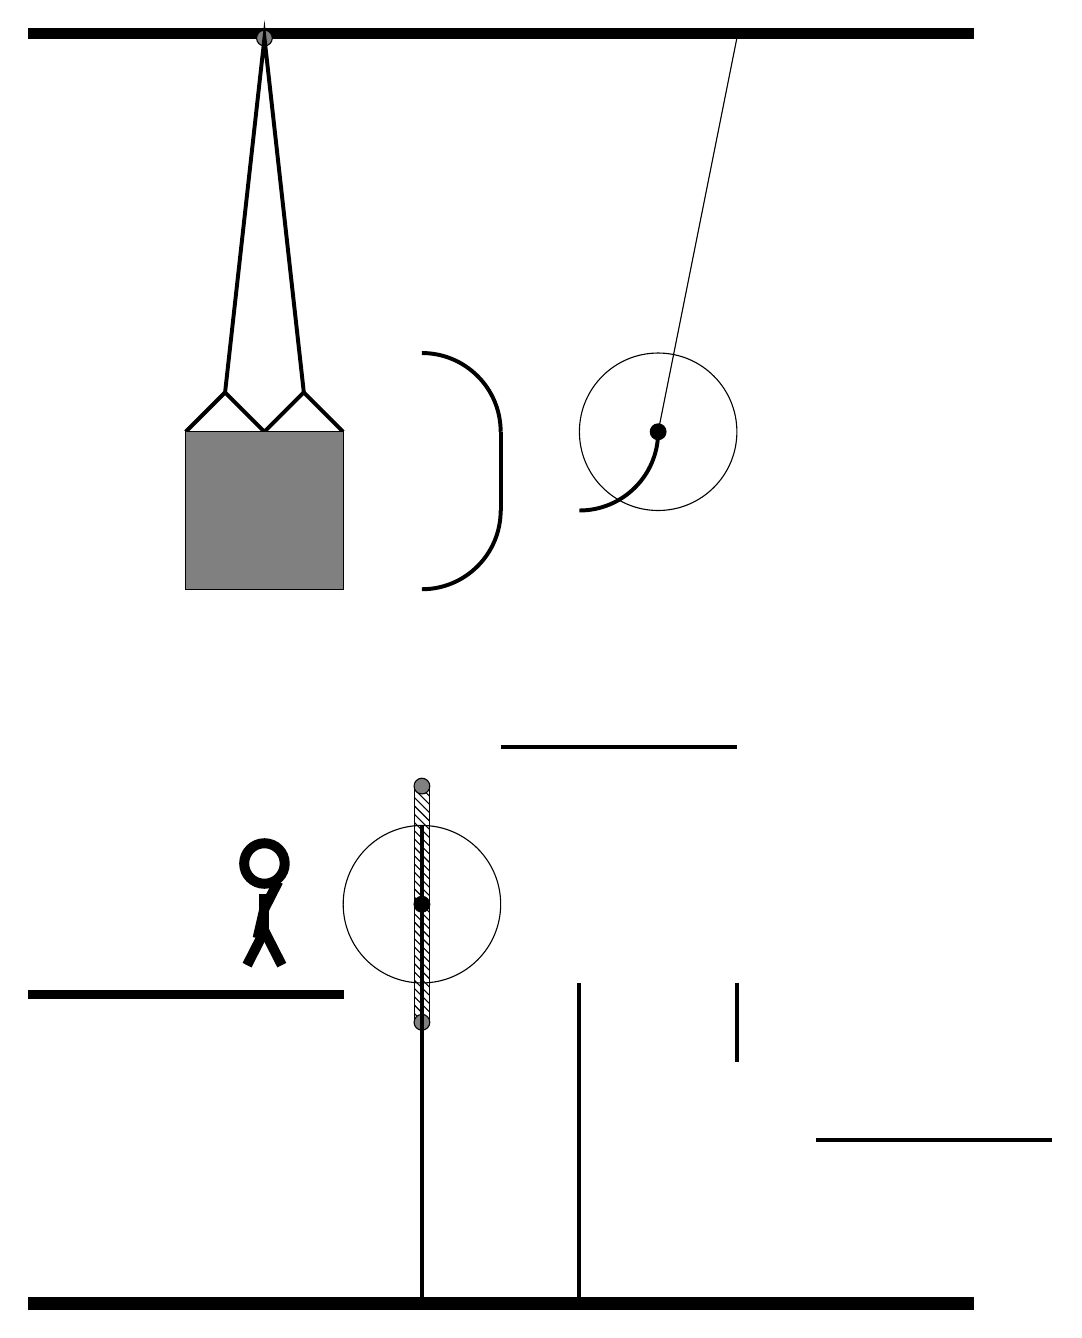
\begin{tikzpicture}
				\draw[fill=black] (-4, 14) rectangle (8, 14.125);
				
				\draw (1,3) circle (1);
				\draw[fill=black] (1,3) circle (0.1);
				\draw[pattern=north west lines, pattern color=black] (0.9,4.5) rectangle (1.1,1.5);
				\draw[fill=black!50] (1,4.5) circle (0.1);
				\draw[fill=black!50] (1,1.5) circle (0.1);
				
				\draw (4,9) circle (1);
				\draw[fill=black] (4,9) circle (0.1);
				\draw (5,14.0) -- (4,9);
				
				\draw[fill=black!50] (-1,14) circle (0.1);
				\draw[line width=0.5mm](-1.5,9.5) -- (-1,14) --  (-0.5,9.5);
				\draw[line width=0.5mm](-2,9) --  (-1.5,9.5) -- (-1,9) -- (-0.5,9.5) -- (0,9);
				\draw[fill=black!50] (-2, 9) rectangle (0, 7);
				
				\draw[line width = 0.5mm] (2,5) -- (5,5);
				\centerarc[line width = 0.5mm](2,4)(90:180:1);
				\draw[line width = 0.5mm] (1,4) -- (1,-2);
				\centerarc[line width = 0.5mm](2,-2)(180:360:1);
				\draw[line width = 0.5mm] (3,-2) -- (3,2);
				\centerarc[line width = 0.5mm](4,2)(0:180:1);
				\draw[line width = 0.5mm] (5,2) -- (5,1);
				\centerarc[line width = 0.5mm](6,1)(180:270:1);
				\draw[line width = 0.5mm] (6,0) -- (9,0);
				\draw[line width = 0.5mm] (1,7) arc (270:360:1);
				\draw[line width = 0.5mm] (2,8) -- (2,9);
				\draw[line width = 0.5mm] (2,9) arc (0:90:1);
				\draw[line width = 0.5mm] (3,8) arc (270:360:1);
				
				\node at (-1, 3) {\scriptsize \Strichmaxerl[10][77][63]};
				\draw[fill=black] (-4, 1.9) rectangle (0, 1.8);
				
				\draw[fill=black] (-4, -2) rectangle (8, -2.15);
			\end{tikzpicture}
		\end{subfigure}
	\end{figure}
		\vspace*{\fill}
\end{document}